\appendix

\section{Empfindlichkeit}

Es sind die drei Aufnahmen des Oszilloskops f�r den Permanentmagneten im Abstand von 1m, 1.5m und 2m zu sehen.

\begin{figure}[H]
\centering
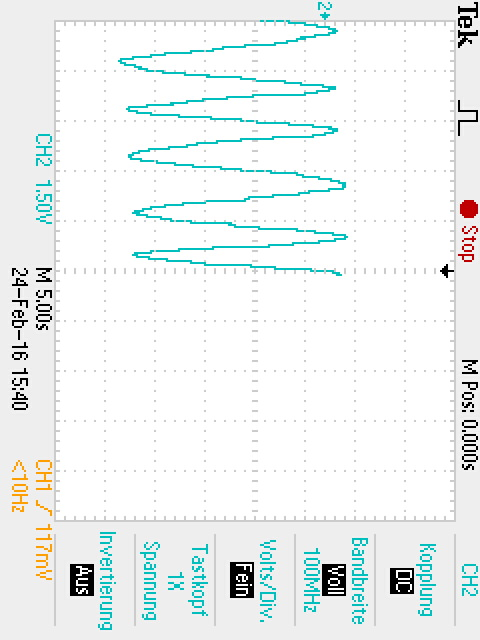
\includegraphics[scale = 0.5,angle=90]{Messungen/TEK0027.JPG}
\caption{Aufnahme der Messspannung bei einem Abstand von 1m}
\label{fig:magnet_1m}
\end{figure}

\begin{figure}[H]
\centering
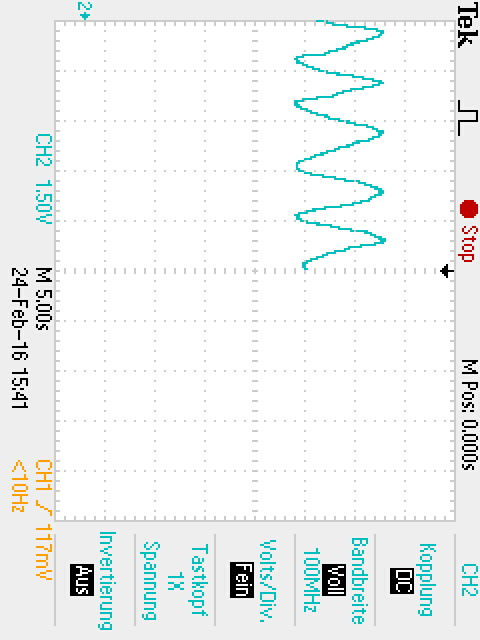
\includegraphics[scale = 0.5,angle=90]{Messungen/TEK0028.JPG}
\caption{Aufnahme der Messspannung bei einem Abstand von 1.5m}
\label{fig:magnet_1.5m}
\end{figure}

\begin{figure}[H]
\centering
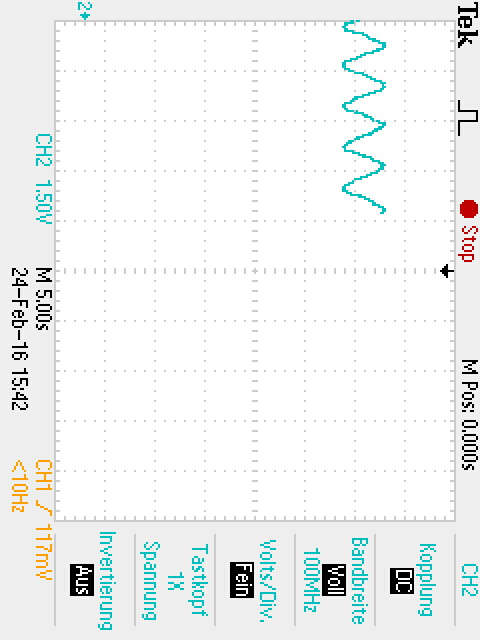
\includegraphics[scale = 0.5,angle=90]{Messungen/TEK0029.JPG}
\caption{Aufnahme der Messspannung bei einem Abstand von 2m}
\label{fig:magent_2m}
\end{figure}

\section{Kalibrierung}
\label{sec:anhang_kalib}
In diesem Abschnitt sind die Aufnahme der Daten f�r die Kalibrierung und deren Fits zu finden.

\begin{figure}[H]
\begin{subfigure}{.48\textwidth}
  \centering
  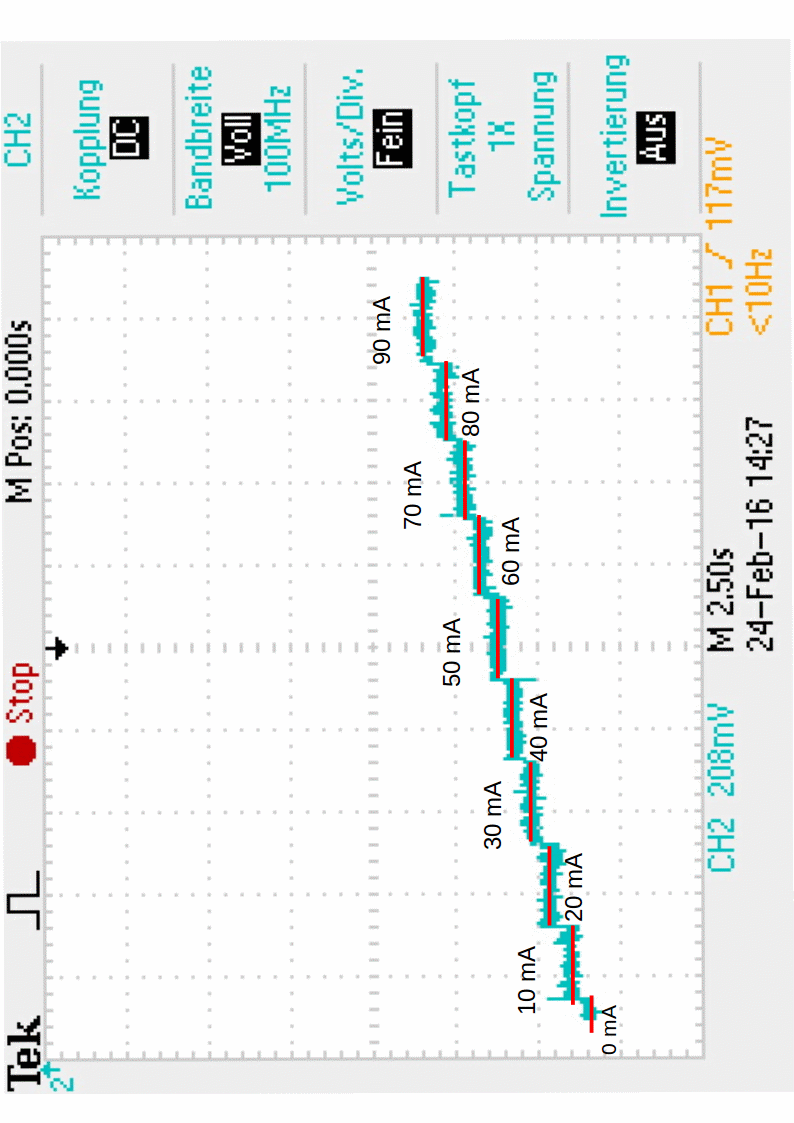
\includegraphics[width=.6\linewidth, angle=-90]{Messungen/bearbeitet/TEK0015.png}
  \caption{Aufnahme des Oszilloskops beim erh�hen des Stroms in 10mA-Schritten.}
  \label{sub_fig:kalib_oszi_1k}
\end{subfigure}%
\begin{subfigure}{.48\textwidth}
  \centering
  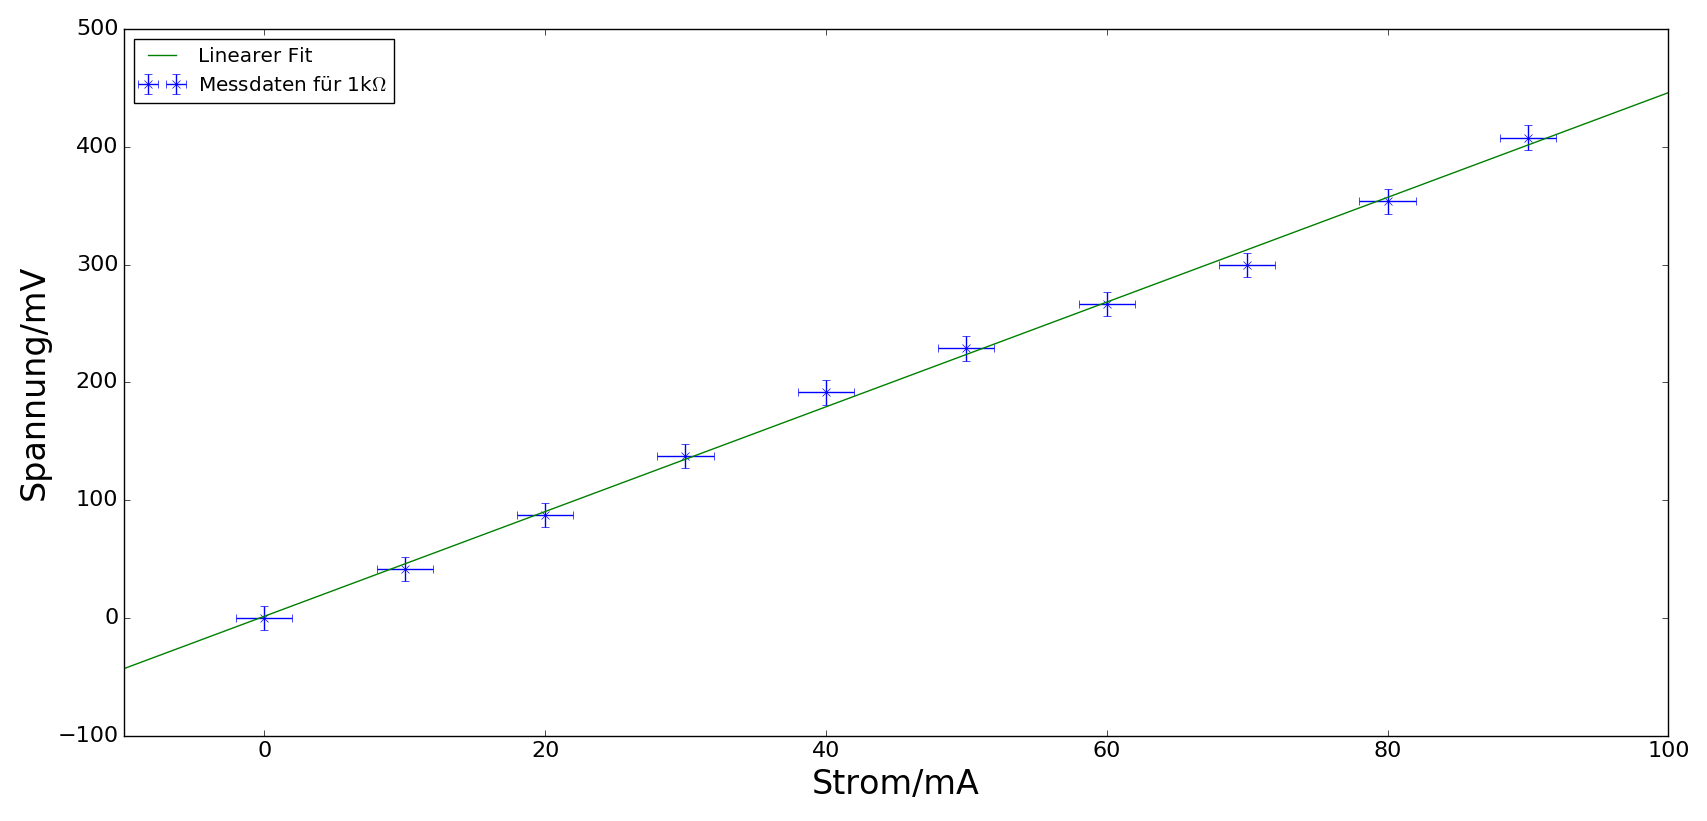
\includegraphics[width=1.1\linewidth]{Fits/1k.png}
  \caption{Linearer Fit f�r den Zusammenhang zwischen Strom und Empfindlichkeit(in Volt)}
  \label{sub_fig:kalib_fit_1k}
\end{subfigure}
\caption{Kalibrierung f�r 1k-Widerstand: F�r den Fit ergab sich ein f�r die Steigung ein Werte von 4.4(8)V/A, f�r den y-Achsenabschnitt ein Wert von 1(4)mA. Das $\chi_{red}^2$ ergibt sich mit 0.5}
\label{fig:kalib_1k}
\end{figure}


\begin{figure}[H]
\begin{subfigure}{.48\textwidth}
  \centering
  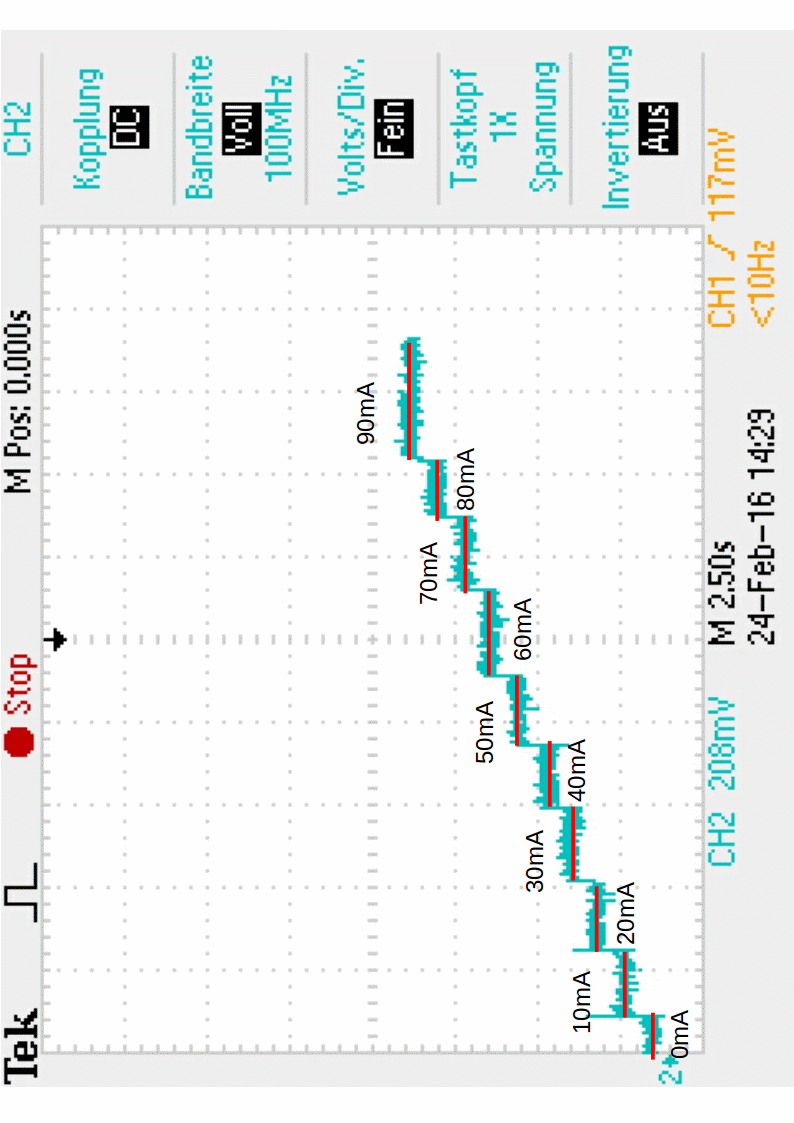
\includegraphics[width=.6\linewidth, angle=-90]{Messungen/bearbeitet/TEK0016.png}
  \caption{Aufnahme des Oszilloskops beim erh�hen des Stroms in 10mA-Schritten.}
  \label{sub_fig:kalib_oszi_1_5k}
\end{subfigure}%
\begin{subfigure}{.48\textwidth}
  \centering
  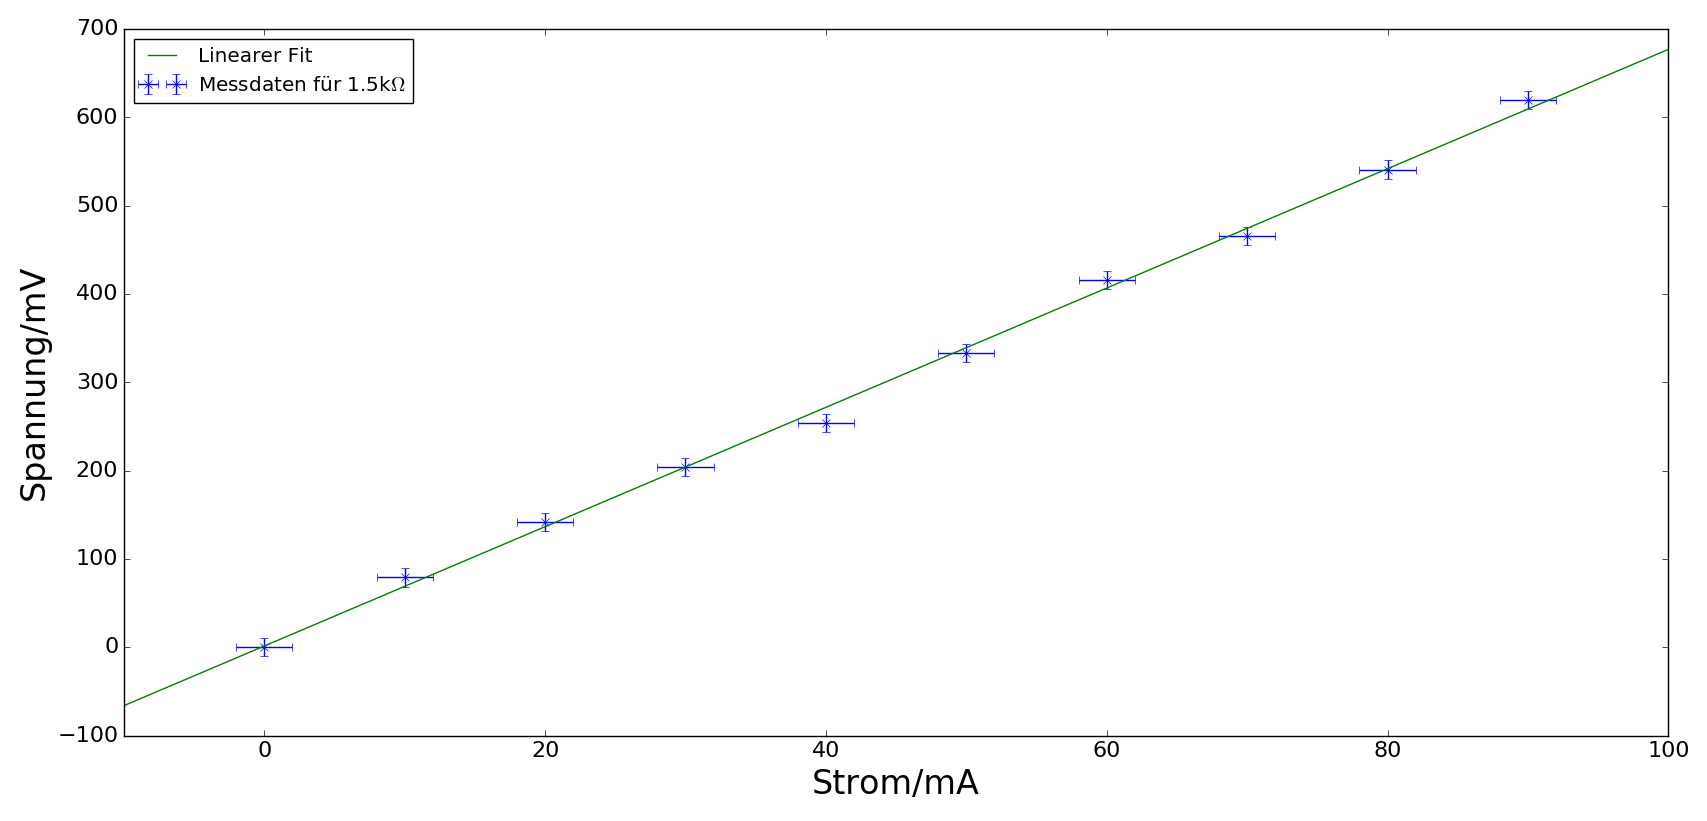
\includegraphics[width=1.1\linewidth]{Fits/1_5k.png}
  \caption{Linearer Fit f�r den Zusammenhang zwischen Strom und Empfindlichkeit(in Volt)}
  \label{sub_fig:kalib_fit_1_5k}
\end{subfigure}
\caption{Kalibrierung f�r 1.5k-Widerstand: F�r den Fit ergab sich ein f�r die Steigung ein Werte von 6.8(1)V/A, f�r den y-Achsenabschnitt ein Wert von 1(5)mA. Das $\chi_{red}^2$ ergibt sich mit 0.87}
\label{fig:kalib_1_5k}
\end{figure}


\begin{figure}[H]
\begin{subfigure}{.48\textwidth}
  \centering
  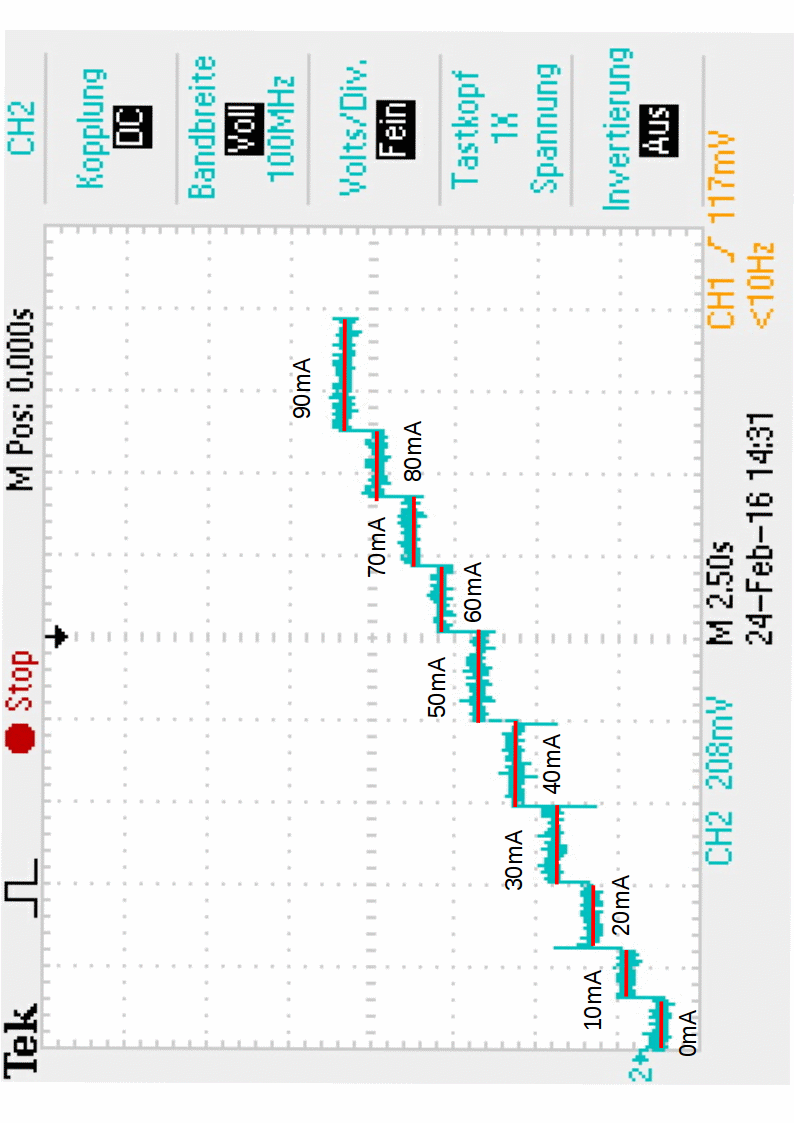
\includegraphics[width=.6\linewidth, angle=-90]{Messungen/bearbeitet/TEK0017.png}
  \caption{Aufnahme des Oszilloskops beim erh�hen des Stroms in 10mA-Schritten.}
  \label{sub_fig:kalib_oszi_2k}
\end{subfigure}%
\begin{subfigure}{.48\textwidth}
  \centering
  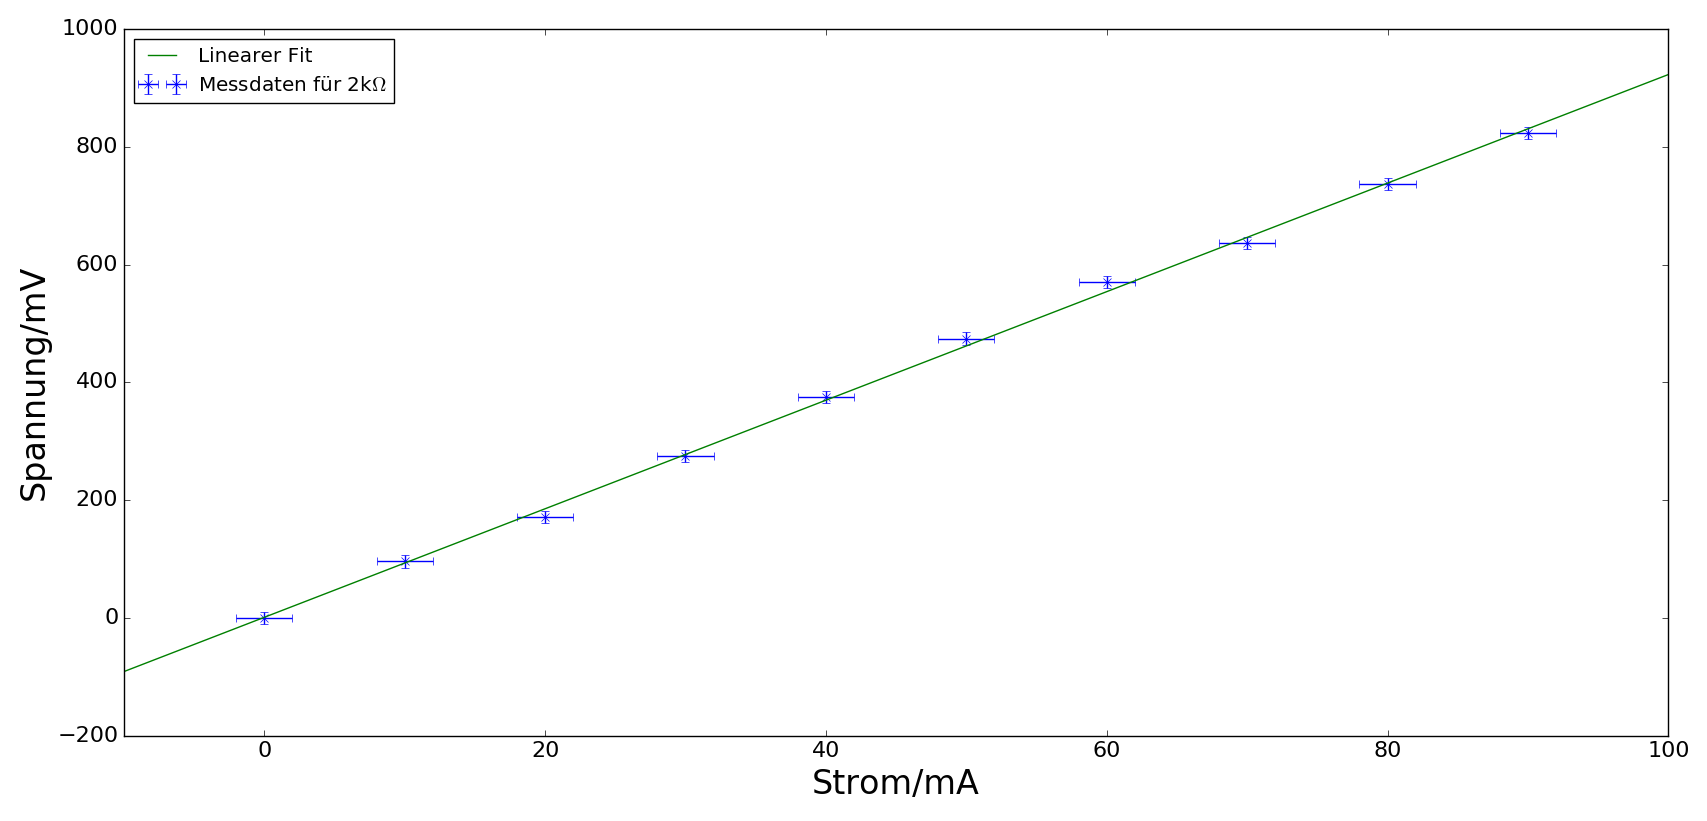
\includegraphics[width=1.1\linewidth]{Fits/2k.png}
  \caption{Linearer Fit f�r den Zusammenhang zwischen Strom und Empfindlichkeit(in Volt)}
  \label{sub_fig:kalib_fit_2k}
\end{subfigure}
\caption{Kalibrierung f�r 2k-Widerstand: F�r den Fit ergab sich ein f�r die Steigung ein Werte von 9.2(1)V/A, f�r den y-Achsenabschnitt ein Wert von 1(5)mA. Das $\chi_{red}^2$ ergibt sich mit 0.93}
\label{fig:kalib_2k}
\end{figure}


\begin{figure}[H]
\begin{subfigure}{.48\textwidth}
  \centering
  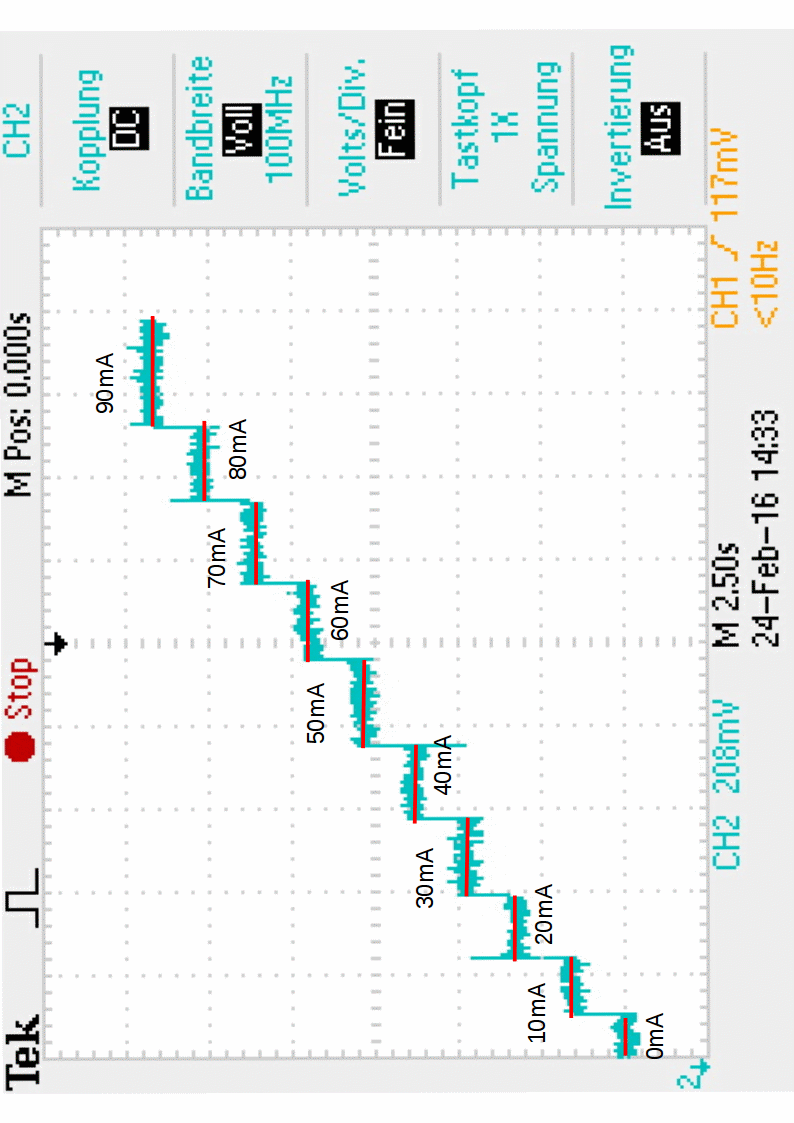
\includegraphics[width=.6\linewidth, angle=-90]{Messungen/bearbeitet/TEK0018.png}
  \caption{Aufnahme des Oszilloskops beim erh�hen des Stroms in 10mA-Schritten.}
  \label{sub_fig:kalib_oszi_3k}
\end{subfigure}%
\begin{subfigure}{.48\textwidth}
  \centering
  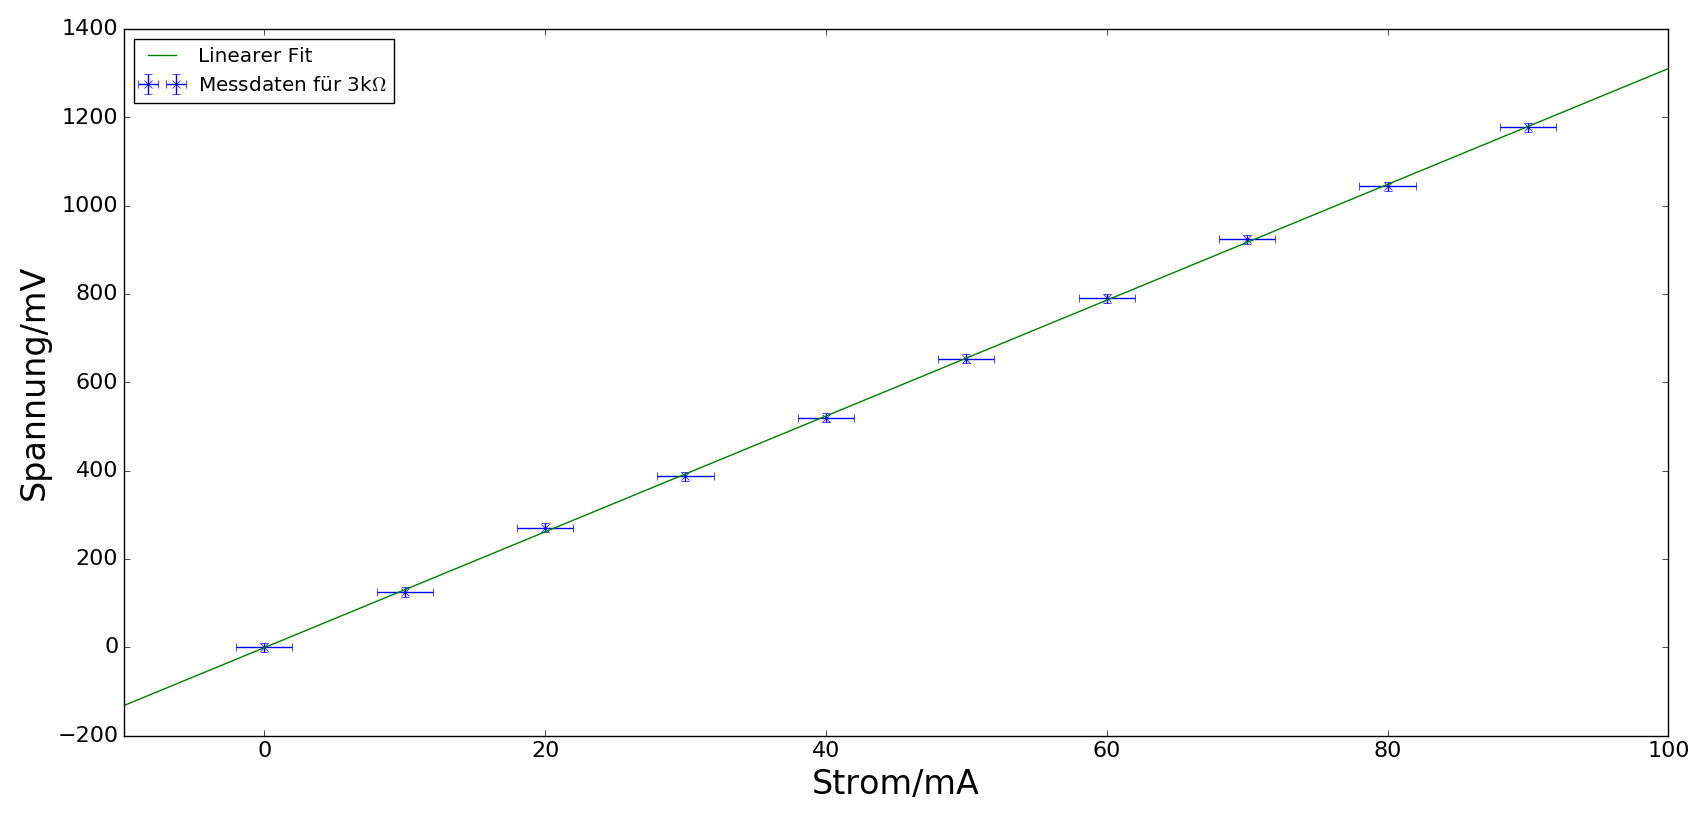
\includegraphics[width=1.1\linewidth]{Fits/3k.png}
  \caption{Linearer Fit f�r den Zusammenhang zwischen Strom und Empfindlichkeit(in Volt)}
  \label{sub_fig:kalib_fit_3k}
\end{subfigure}
\caption{Kalibrierung f�r 3k-Widerstand: F�r den Fit ergab sich ein f�r die Steigung ein Werte von 13.11(6)V/A, f�r den y-Achsenabschnitt ein Wert von -1(3)mA. Das $\chi_{red}^2$ ergibt sich mit 0.28}
\label{fig:kalib_3k}
\end{figure}


\begin{figure}[H]
\begin{subfigure}{.48\textwidth}
  \centering
  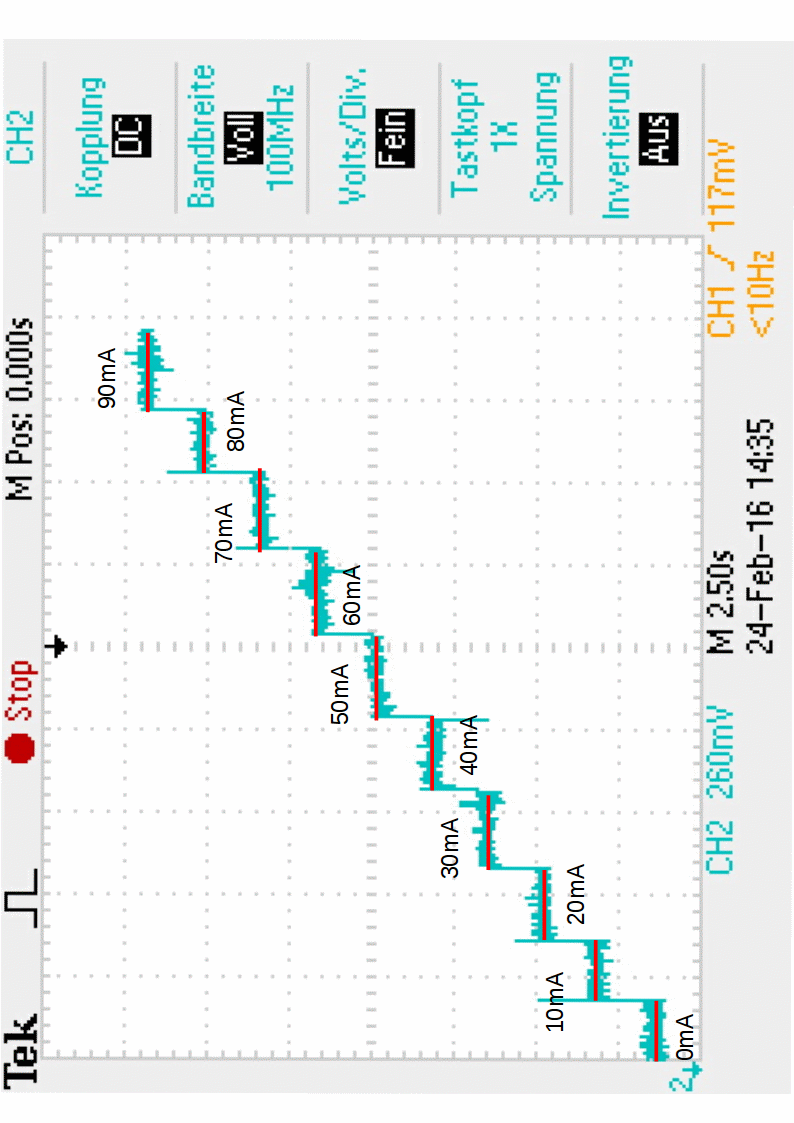
\includegraphics[width=.6\linewidth, angle=-90]{Messungen/bearbeitet/TEK0019.png}
  \caption{Aufnahme des Oszilloskops beim erh�hen des Stroms in 10mA-Schritten.}
  \label{sub_fig:kalib_oszi_4k}
\end{subfigure}%
\begin{subfigure}{.48\textwidth}
  \centering
  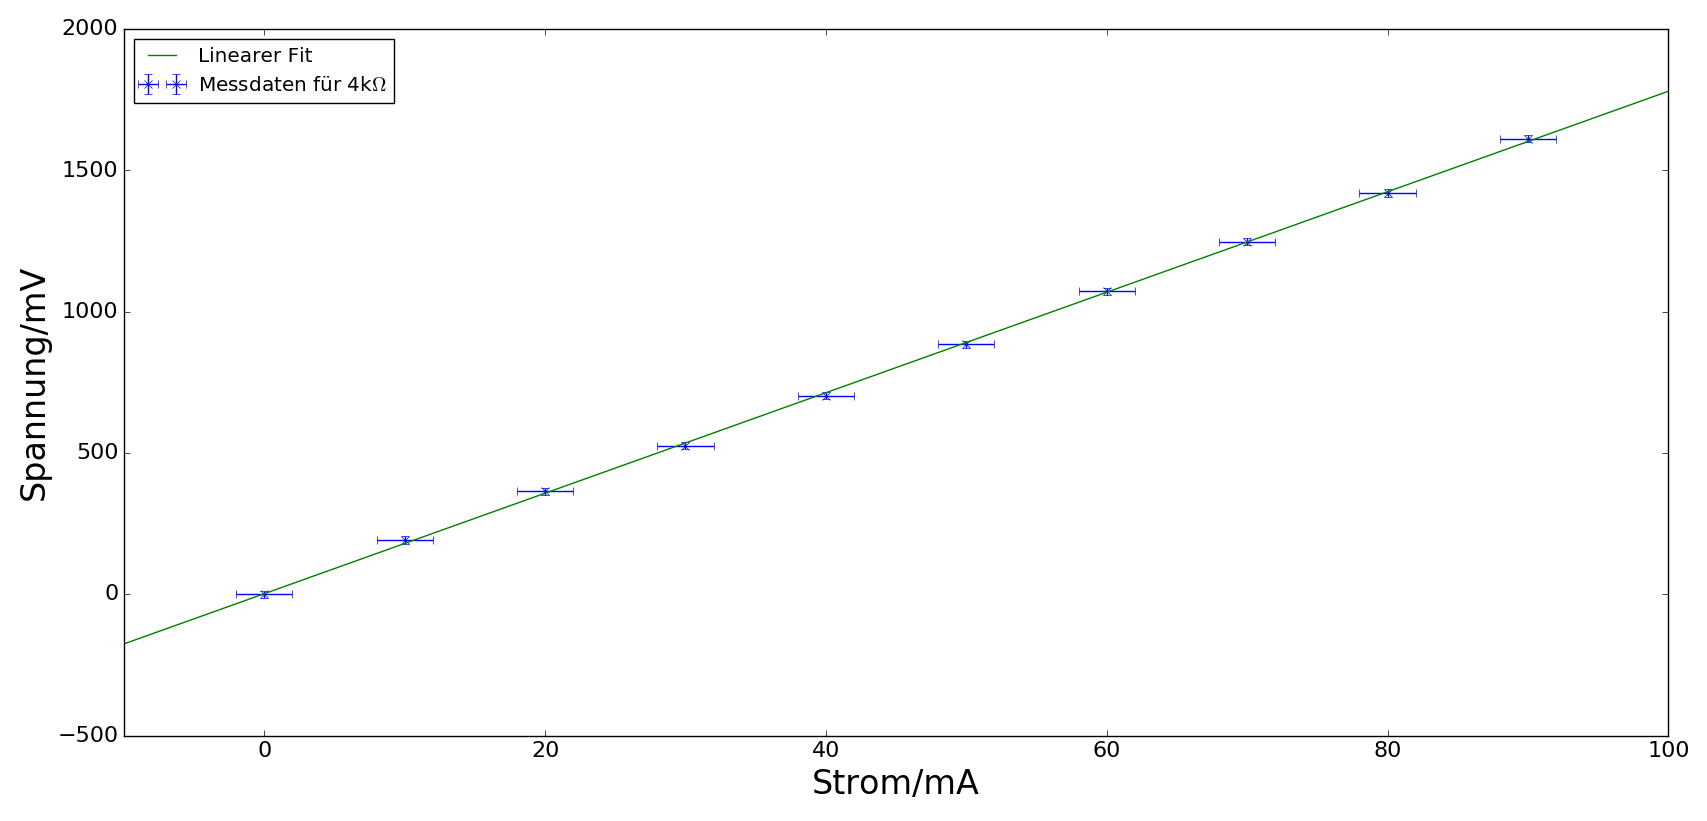
\includegraphics[width=1.1\linewidth]{Fits/4k.png}
  \caption{Linearer Fit f�r den Zusammenhang zwischen Strom und Empfindlichkeit(in Volt)}
  \label{sub_fig:kalib_fit_4k}
\end{subfigure}
\caption{Kalibrierung f�r 4k-Widerstand: F�r den Fit ergab sich ein f�r die Steigung ein Werte von 17.8(1)V/A, f�r den y-Achsenabschnitt ein Wert von 2(5)mA. Das $\chi_{red}^2$ ergibt sich mit 0.45}
\label{fig:kalib_4k}
\end{figure}


\begin{figure}[H]
\begin{subfigure}{.48\textwidth}
  \centering
  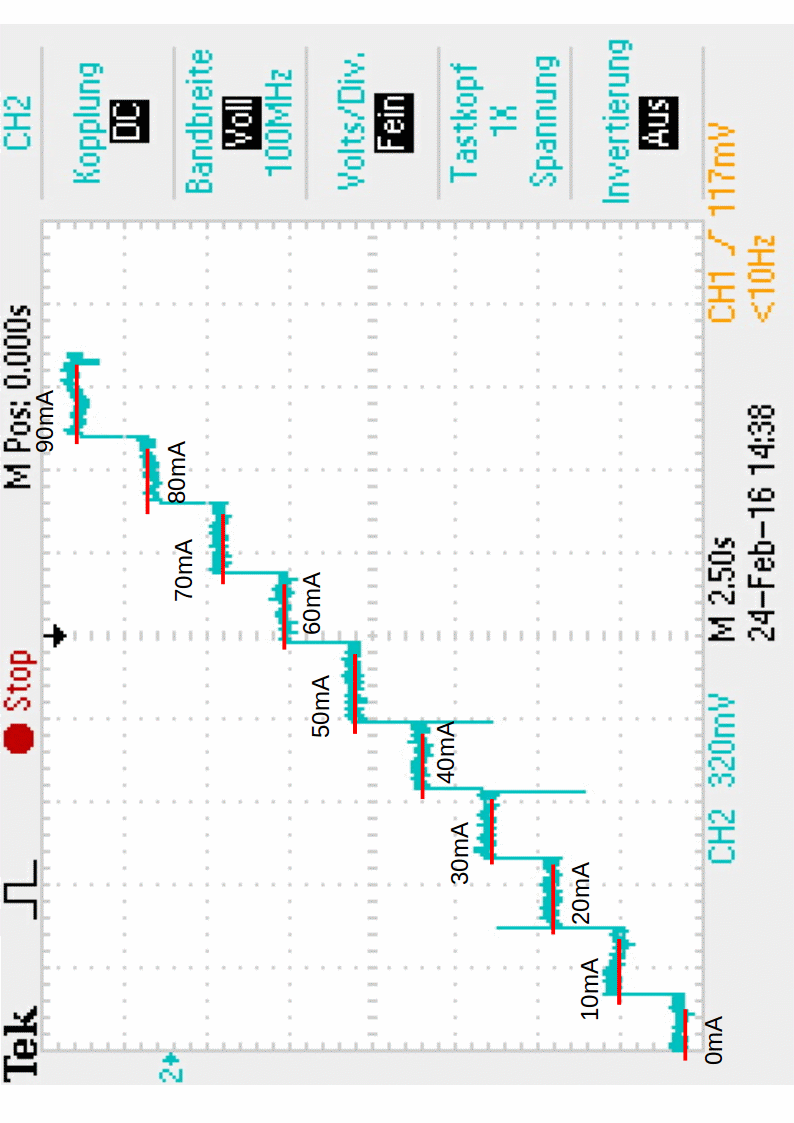
\includegraphics[width=.6\linewidth, angle=-90]{Messungen/bearbeitet/TEK0020.png}
  \caption{Aufnahme des Oszilloskops beim erh�hen des Stroms in 10mA-Schritten.}
  \label{sub_fig:kalib_oszi_6k}
\end{subfigure}%
\begin{subfigure}{.48\textwidth}
  \centering
  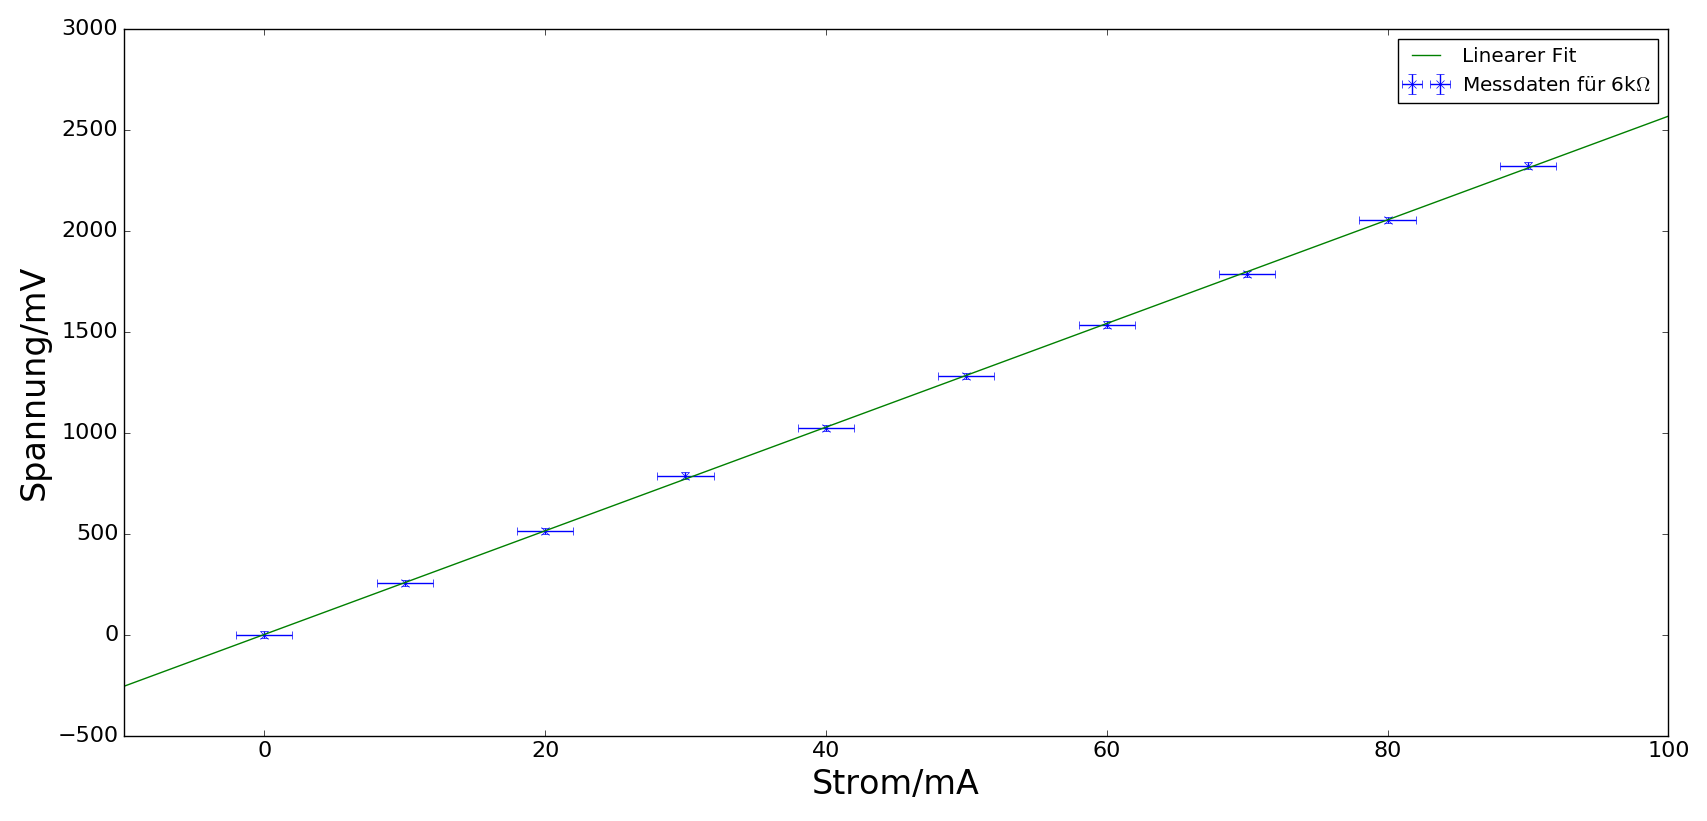
\includegraphics[width=1.1\linewidth]{Fits/6k.png}
  \caption{Linearer Fit f�r den Zusammenhang zwischen Strom und Empfindlichkeit(in Volt)}
  \label{sub_fig:kalib_fit_6k}
\end{subfigure}
\caption{Kalibrierung f�r 6k-Widerstand: F�r den Fit ergab sich ein f�r die Steigung ein Werte von 25.7(1)V/A, f�r den y-Achsenabschnitt ein Wert von 0(5)mA. Das $\chi_{red}^2$ ergibt sich mit 0.3}
\label{fig:kalib_6k}
\end{figure}


\begin{figure}[H]
\begin{subfigure}{.48\textwidth}
  \centering
  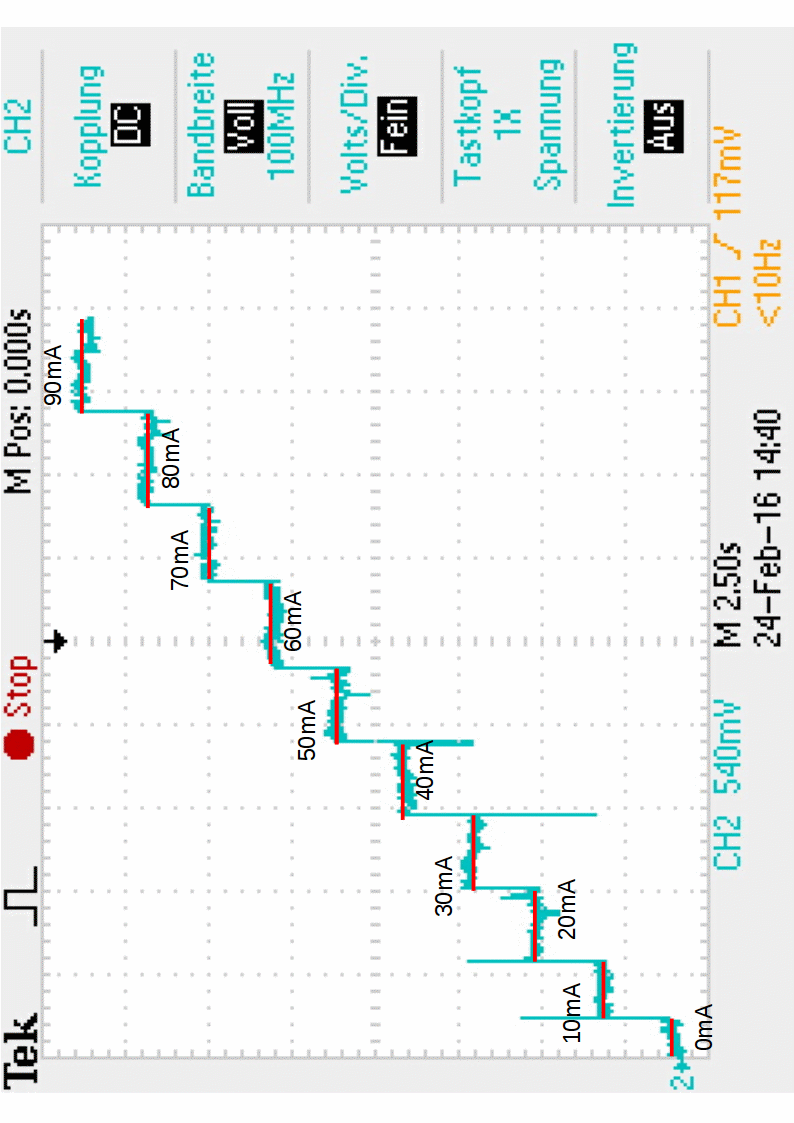
\includegraphics[width=.6\linewidth, angle=-90]{Messungen/bearbeitet/TEK0021.png}
  \caption{Aufnahme des Oszilloskops beim erh�hen des Stroms in 10mA-Schritten.}
  \label{sub_fig:kalib_oszi_10k}
\end{subfigure}%
\begin{subfigure}{.48\textwidth}
  \centering
  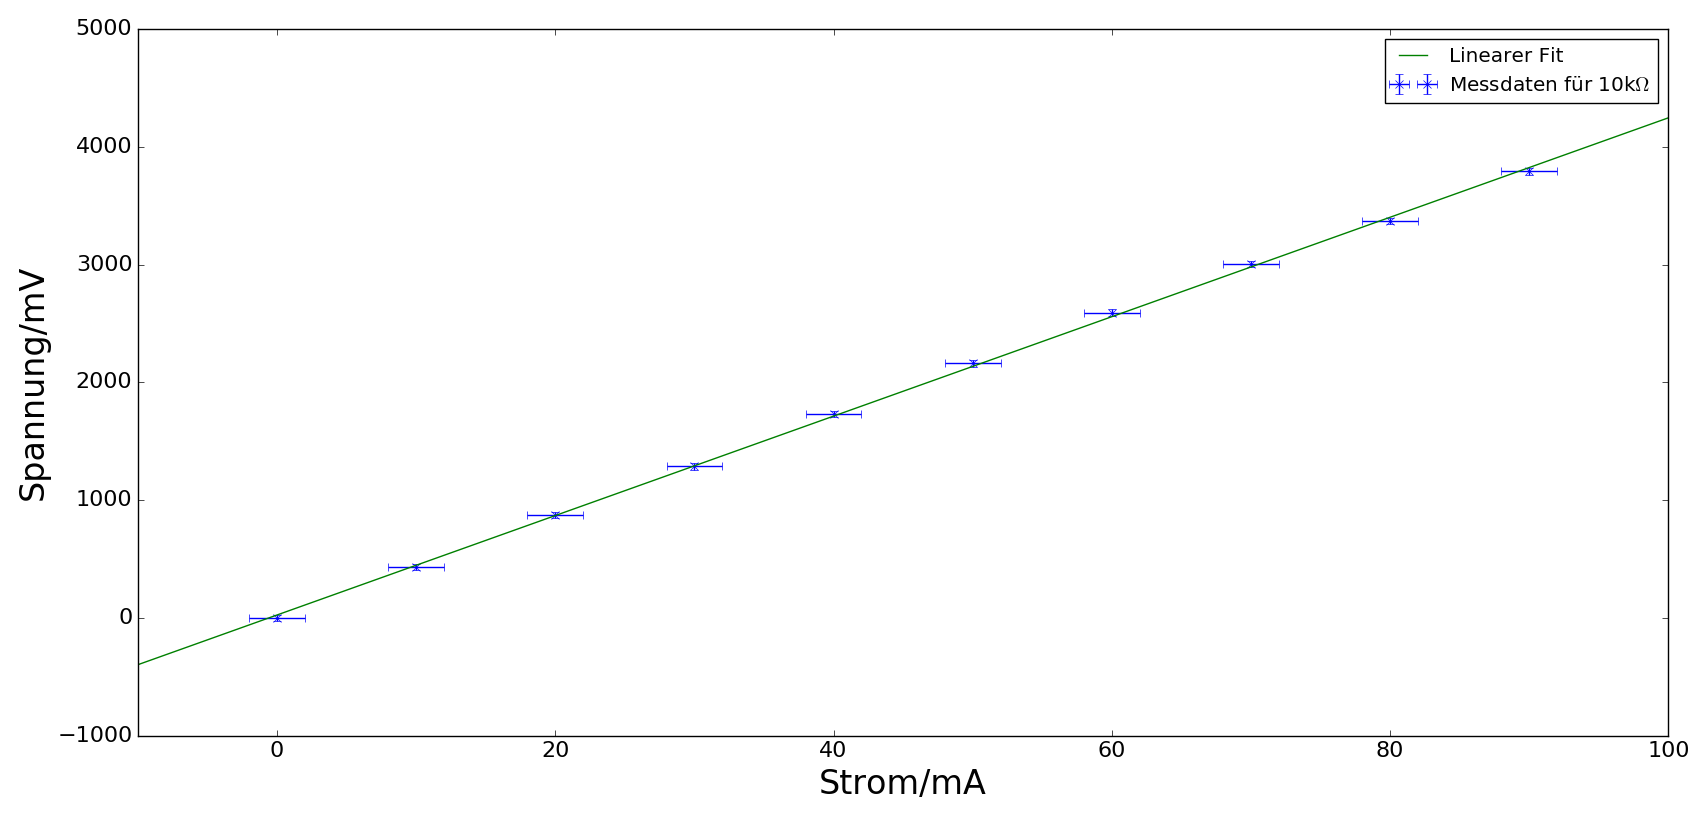
\includegraphics[width=1.1\linewidth]{Fits/10k.png}
  \caption{Linearer Fit f�r den Zusammenhang zwischen Strom und Empfindlichkeit(in Volt)}
  \label{sub_fig:kalib_fit_10k}
\end{subfigure}
\caption{Kalibrierung f�r 10k-Widerstand: F�r den Fit ergab sich ein f�r die Steigung ein Werte von 42.2(3)V/A, f�r den y-Achsenabschnitt ein Wert von 23(15)mA. Das $\chi_{red}^2$ ergibt sich mit 0.95}
\label{fig:kalib_10k}
\end{figure}


\begin{figure}[H]
\begin{subfigure}{.48\textwidth}
  \centering
  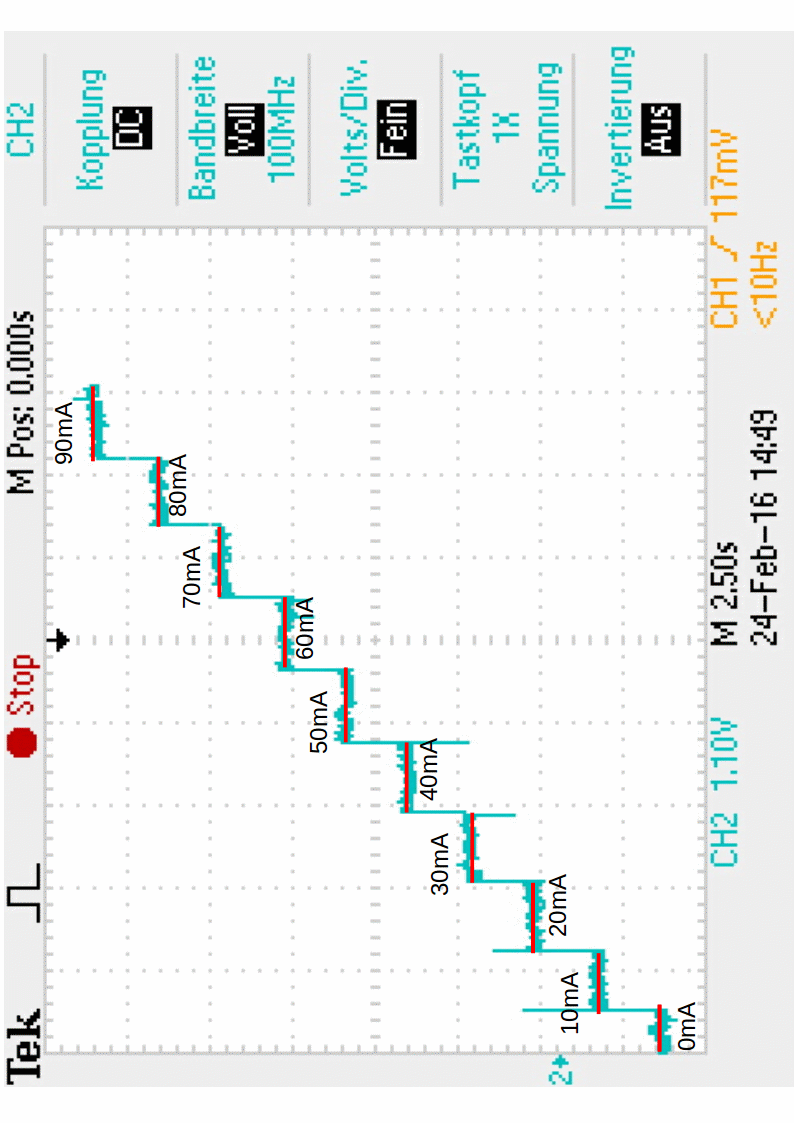
\includegraphics[width=.6\linewidth, angle=-90]{Messungen/bearbeitet/TEK0022.png}
  \caption{Aufnahme des Oszilloskops beim erh�hen des Stroms in 10mA-Schritten.}
  \label{sub_fig:kalib_oszi_20k}
\end{subfigure}%
\begin{subfigure}{.48\textwidth}
  \centering
  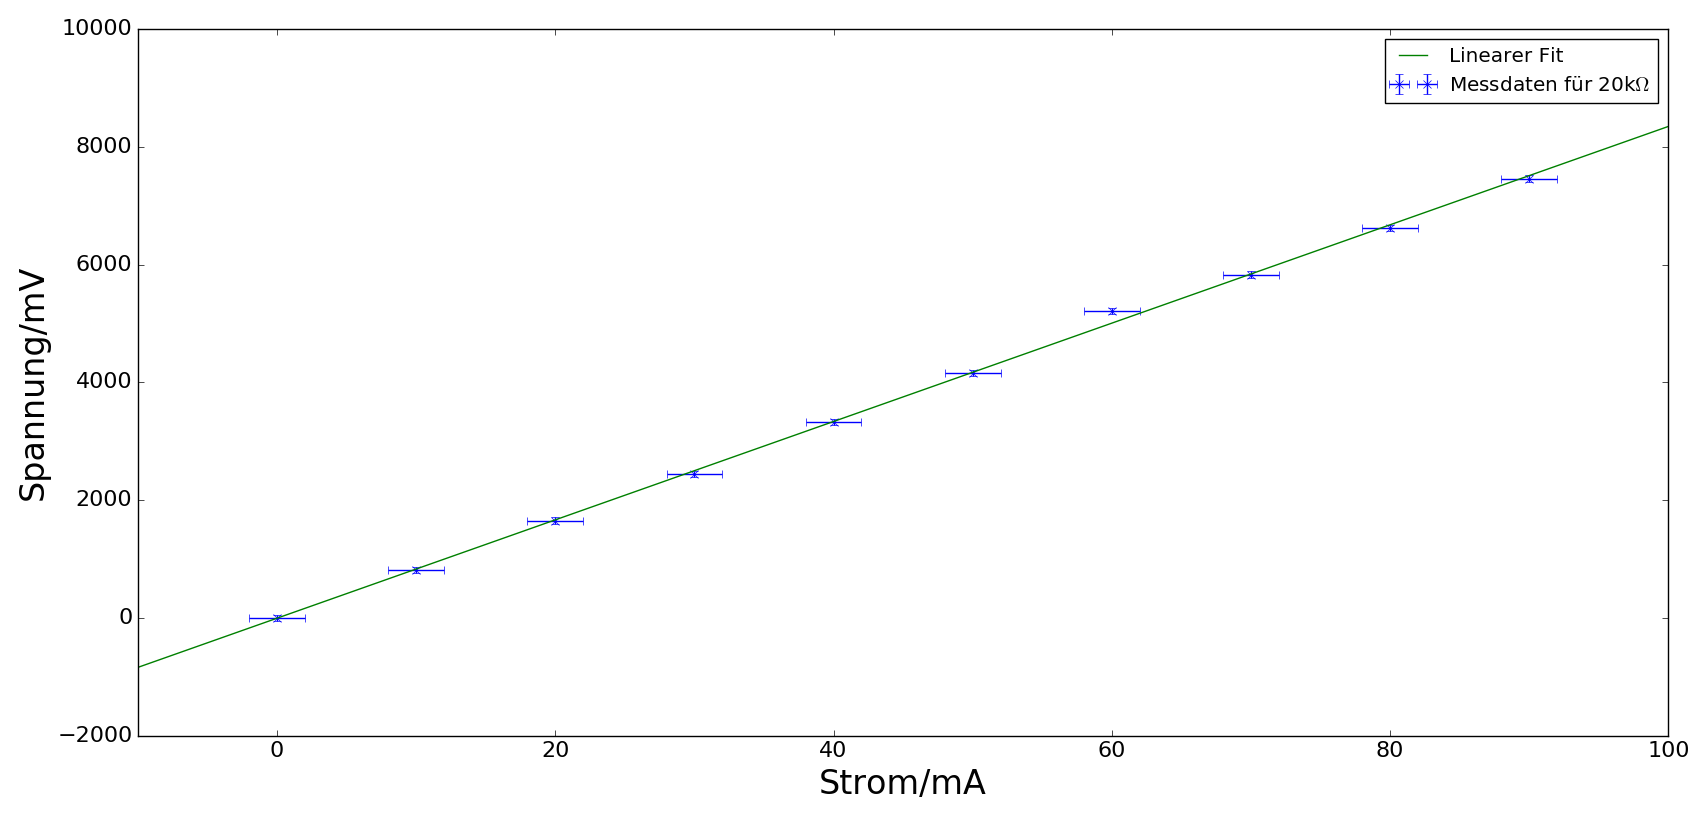
\includegraphics[width=1.1\linewidth]{Fits/20k.png}
  \caption{Linearer Fit f�r den Zusammenhang zwischen Strom und Empfindlichkeit(in Volt)}
  \label{sub_fig:kalib_fit_20k}
\end{subfigure}
\caption{Kalibrierung f�r 20k-Widerstand: F�r den Fit ergab sich ein f�r die Steigung ein Werte von 83.5(9)V/A, f�r den y-Achsenabschnitt ein Wert von -8(48)mA. Das $\chi_{red}^2$ ergibt sich mit 2.21}
\label{fig:kalib_20k}
\end{figure}

%\section{Jupyter-Notebook}

%\includepdf[pages=-]{ipython_notebook_pdf/python_squid_datenanalyse.pdf}